% Talk: AI in mobile apps. Compile: latexmk -xelatex ai-in-mobile-apps.tex
\documentclass[10pt,aspectratio=169,t]{beamer}
\usetheme{upbminimal}

\course{AI in mobile apps}
\decklabel{Talk}
\title{AI in mobile apps}
\subtitle{On-device ML, LLMs, RAG and MCP}
\author{Dinu-Ștefan Rusu}
\institute{CodingShadows · rusudinu.ro}
\date{2026}

\begin{document}

\titleframe

\begin{frame}[eyebrow=Speaker]{Who is talking}
  \vskip 2mm
  \begin{grid}[2]
    \cell[\faUserTie]{Dinu-Ștefan Rusu}{Founder and senior engineer at CodingShadows. I build mobile products for clients and teach mobile development at university.}
    \cell[\faMobile]{Building for next-gen mobile experiences}{Flutter and native apps in production, plus the machine learning parts that sit behind them.}
  \end{grid}
  \vskip 6mm
  \kv{Where to find me}{\link{https://rusudinu.ro}{rusudinu.ro} · \link{https://codingshadows.com}{codingshadows.com}}
  \note{Keep this short. Say one sentence about the product the examples come from, a food scanning app, so the room knows the screenshots are from something real and not a toy.}
\end{frame}

\begin{frame}[eyebrow=Today]{What this talk covers}
  \vskip 2mm
  \begin{grid}[3]
    \cell[\faCamera]{On-device ML}{ML Kit text recognition and barcodes. What the phone does with no network at all.}
    \cell[\faComments]{Talking to a model}{Hosted or local, the request shape, streaming, and where the key may live.}
    \cell[\faDatabase]{Retrieval}{Embeddings, distance, approximate search, chunking, one real index.}
    \cell[\faWrench]{Tools and MCP}{Function calling, Model Context Protocol servers, three notebooks.}
    \cell[\faLock]{Security}{Input checks, token budgets, human approval, output guardrails.}
  \end{grid}
  \note{Tell the room the deck is demo driven and that every code path shown also exists in a notebook they can clone. Ask who already ships something with a model in it, so you know how fast to go through Part 1.}
\end{frame}

\divider{Part 1 · On-device ML}{The camera is already a sensor}[ML Kit text recognition, barcodes, and what never leaves the phone]

\begin{frame}[eyebrow=On-device]{What runs on the phone}
  \vskip 2mm
  \begin{grid}[3]
    \cell[\faFont]{Text recognition}{Latin, Chinese, Japanese, Korean and Devanagari scripts. Returns blocks, lines and elements with bounding boxes.}
    \cell[\faBarcode]{Barcode scanning}{Most one- and two-dimensional formats. Parses known payloads such as URLs, contacts and Wi-Fi.}
    \cell[\faIcon{id-badge}]{Face and pose}{Landmarks, contours and body keypoints at frame rate, with no server and no upload.}
    \cell[\faTags]{Image labeling}{Generic labels from a bundled model, or your own model exported to TensorFlow Lite.}
    \cell[\faLanguage]{Translation}{Small language packs downloaded once, then translation with the network off.}
    \cell[\faIcon{file-alt}]{Document scanner}{Edge detection, perspective correction and a clean page image handed back to the app.}
  \end{grid}
  \note{The point of this grid is availability, not novelty. Most of the room already has these APIs on the device and has never called them. Name the two they are most likely to need: text recognition and barcodes.}
\end{frame}

\begin{frame}[eyebrow=On-device]{Text recognition returns text, not meaning}
  \vskip 1mm
  \begin{center}
    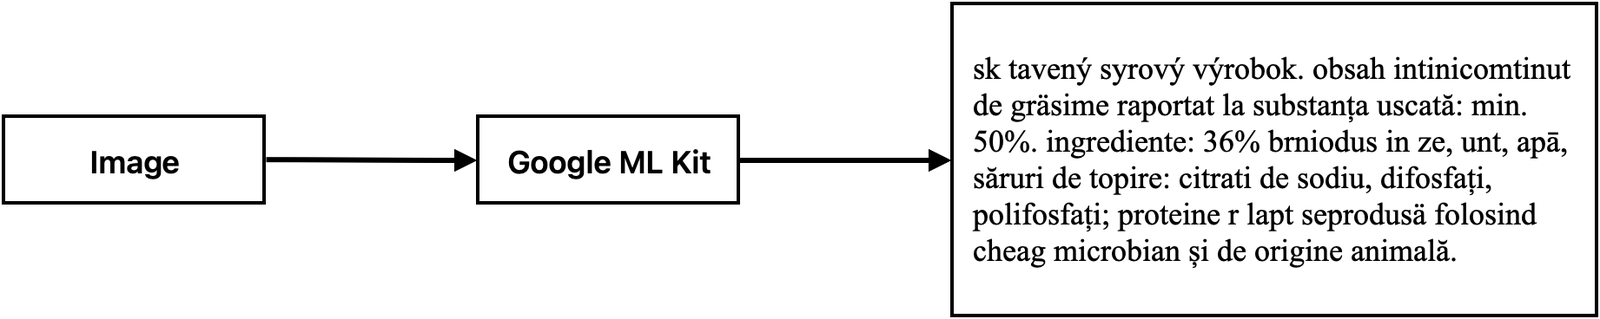
\includegraphics[width=\textwidth,height=27mm,keepaspectratio]{images/onia-s07-3.png}
  \end{center}
  \vskip 2mm
  \muted{The model reads a food label and hands back one string: broken words, missing diacritics, wrong characters, no structure. The app wanted a list of additive codes.}
  \begin{takeaway}{Recognition is the cheap half of the job.}
    Everything after it is ordinary code that you write, test and own.
  \end{takeaway}
  \note{Read two lines of the recognized text out loud so the room hears how bad it is. This is the moment where people stop expecting the model to do the whole task.}
\end{frame}

\begin{frame}[fragile,eyebrow=On-device]{Reading text from a camera frame}
\begin{kotlin}
val options = TextRecognizerOptions.DEFAULT_OPTIONS
val recognizer = TextRecognition.getClient(options)

val image = InputImage.fromMediaImage(mediaImage, rotationDegrees)
recognizer.process(image)
    .addOnSuccessListener { result ->
        val lines = result.textBlocks.flatMap { it.lines }
        handle(lines.map { it.text })
    }
    .addOnFailureListener { error -> report(error) }
\end{kotlin}
  \vskip 1mm
  \muted{The same call exists on iOS and through the Flutter plugin. Close the image when you are done, or the camera pipeline stalls after a few frames.}
  \note{Point at the bounding boxes you are throwing away here. On a nutrition label the geometry tells you which text belongs to the ingredient list, and that alone removes most of the noise.}
\end{frame}

\begin{frame}[eyebrow=On-device]{From raw text to additive codes}
  \vskip 1mm
  \begin{center}
    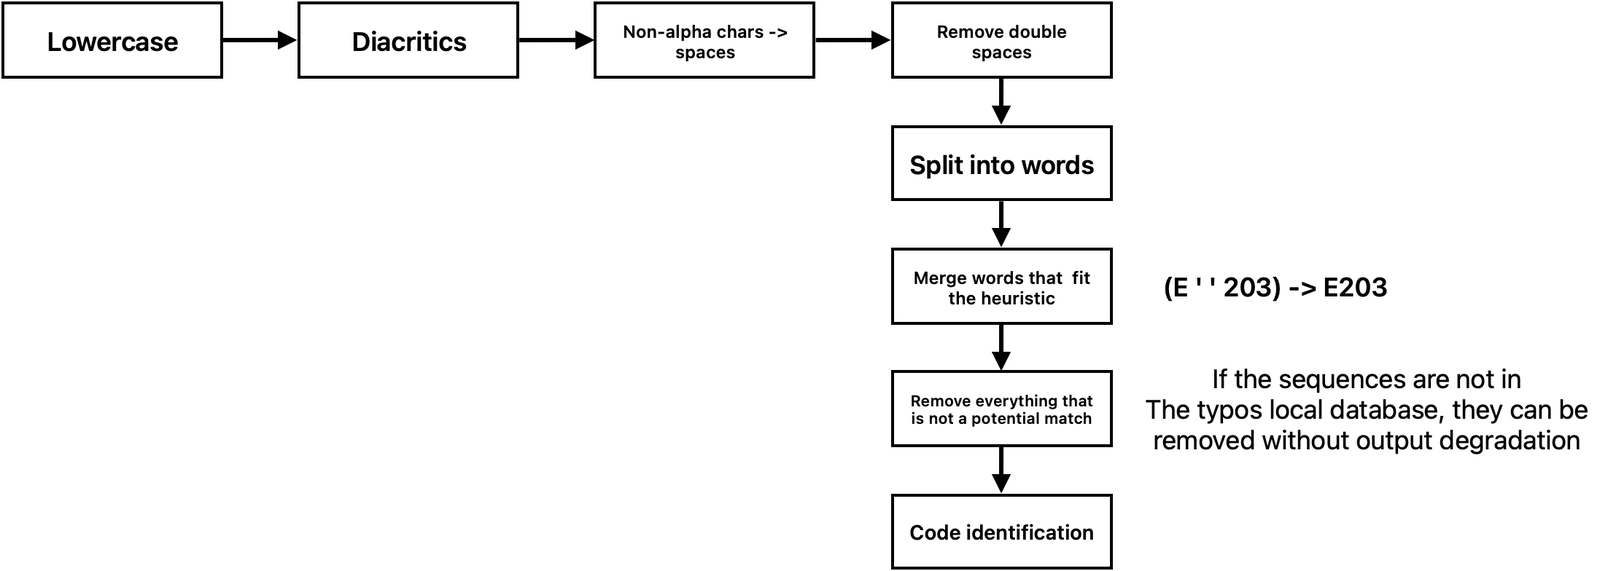
\includegraphics[width=\textwidth,height=31mm,keepaspectratio]{images/onia-s11-1.png}
  \end{center}
  \vskip 1mm
  \muted{Lowercase, strip diacritics, replace every non-letter with a space, split, then merge fragments that fit the shape of a code. What is left is matched against a local list.}
  \begin{takeaway}{Normalize first, match second.}
    A short deterministic pipeline recovers most of what the recognizer got wrong.
  \end{takeaway}
  \note{Explain the merge heuristic with one example: E, space, space, 203 becomes E203. Then mention the overlapped chunks and character n-grams that follow, which catch codes split across two recognized lines.}
\end{frame}

\begin{frame}[eyebrow=Cloud]{On the device or in the cloud}
  \vskip 1mm
  \muted{Sent to a hosted multimodal model, the same photo comes back as the finished list of codes. One call replaces the whole pipeline above.}
  \vskip 2mm
  {\usebeamerfont{small}\begin{tabular}{@{}lllp{56mm}@{}}
    \toprule
    \thead{Question} & \thead{On device} & \thead{Cloud} & \multicolumn{1}{l@{}}{\thead{What decides it}} \\
    \midrule
    Latency       & tens of ms     & hundreds of ms & a camera preview needs the device \\
    Works offline & yes            & no             & shops and basements have no signal \\
    Cost per call & zero           & per token      & a scanner runs constantly \\
    Privacy       & nothing leaves & image uploaded & pictures of documents and people \\
    \bottomrule
  \end{tabular}}
  \begin{takeaway}{Use both.}
    Recognize on the device, escalate to the cloud only when the local result is empty.
  \end{takeaway}
  \note{Say plainly that the cloud path was shorter to build and harder to guarantee. It fails differently too: instead of missing a code it can invent one, which is much worse for a health feature. Ask the room what fraction of scans really need it.}
\end{frame}

\begin{frame}[eyebrow=On-device]{The whole pipeline on one slide}
  \vskip 2mm
  \begin{center}
    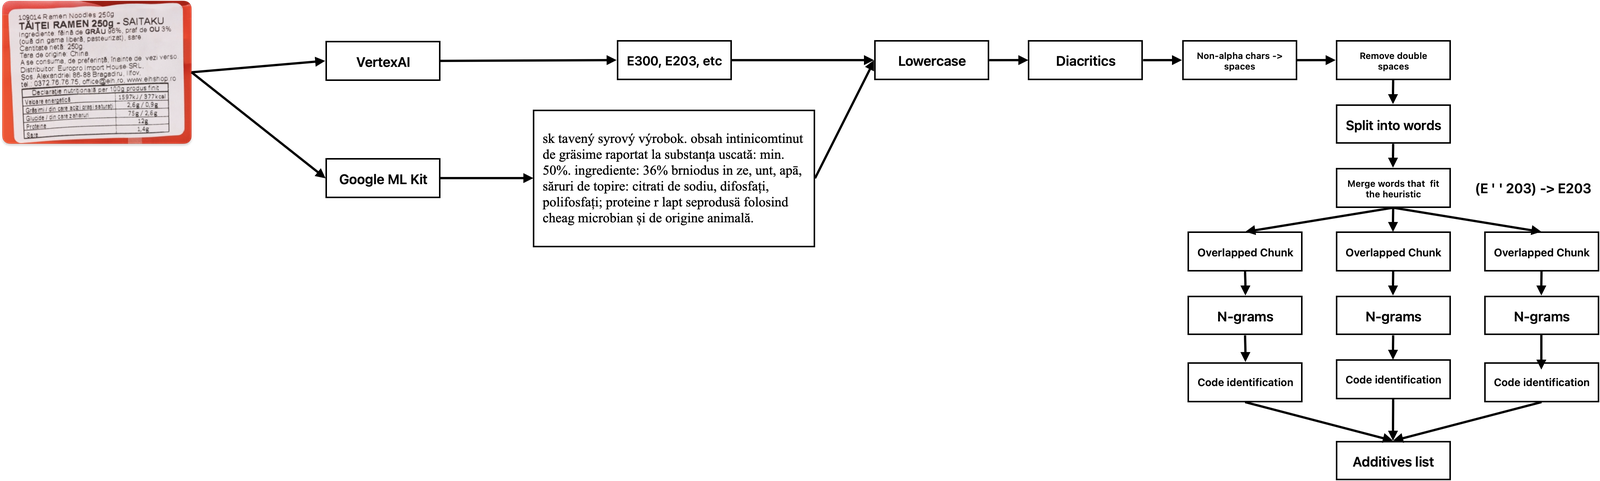
\includegraphics[width=\textwidth,height=38mm,keepaspectratio]{images/onia-s16-1.png}
  \end{center}
  \vskip 3mm
  \muted{One photo, two recognizers, one normalization chain, one local lookup. Both branches return the same shape of result, so the rest of the app does not care which answered.}
  \note{This is the recap of Part 1. Stress the last sentence: one result type makes it possible to switch the branch behind a flag and measure the difference in production.}
\end{frame}

\divider{Part 2 · Talking to a model}{A chat box is a second user interface}[Hosted or local, the request shape, streaming, and where keys live]

\begin{frame}[eyebrow=Conversation]{Chat is a second way into the same app}
  \vskip 1mm
  \begin{center}
    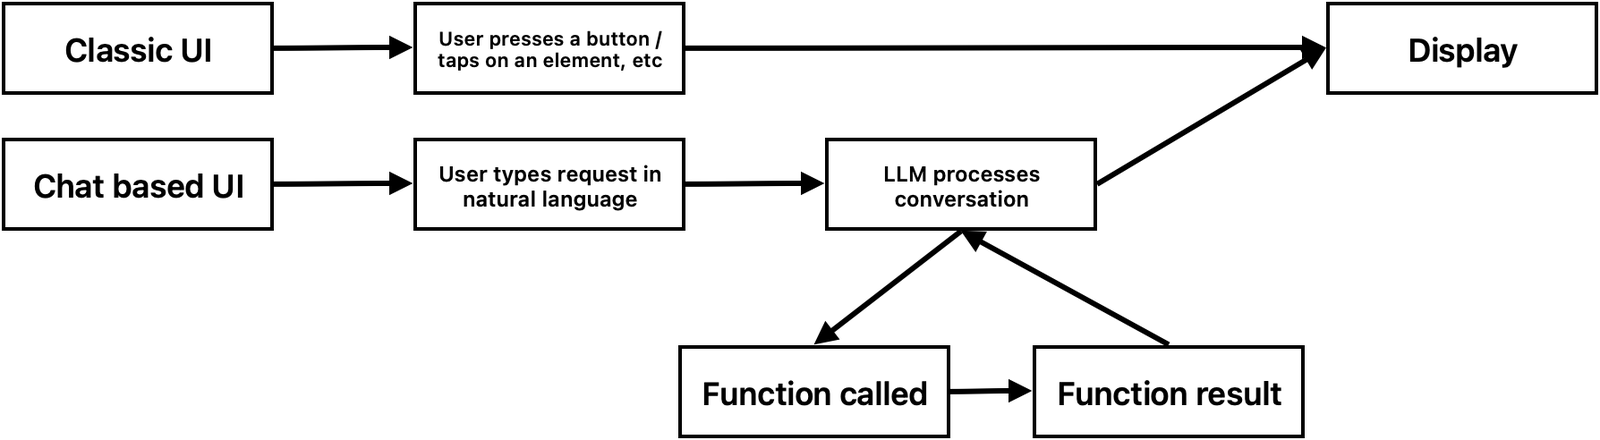
\includegraphics[width=\textwidth,height=26mm,keepaspectratio]{images/onia-s17-1.png}
  \end{center}
  \vskip 2mm
  \muted{The classic path is a tap that calls a function and draws a screen. The chat path is a sentence that the model turns into the same call. Both end in the same display code.}
  \begin{takeaway}{You are not building a chatbot.}
    You are adding a second entry point to functions your app already has.
  \end{takeaway}
  \note{This framing sells the feature internally. Nobody approves a chatbot, but everybody approves a faster way to reach a screen that is four taps deep.}
\end{frame}

\begin{frame}[eyebrow=Conversation]{What it looks like on the phone}
  \begin{columns}[T]
    \begin{column}{0.58\textwidth}
      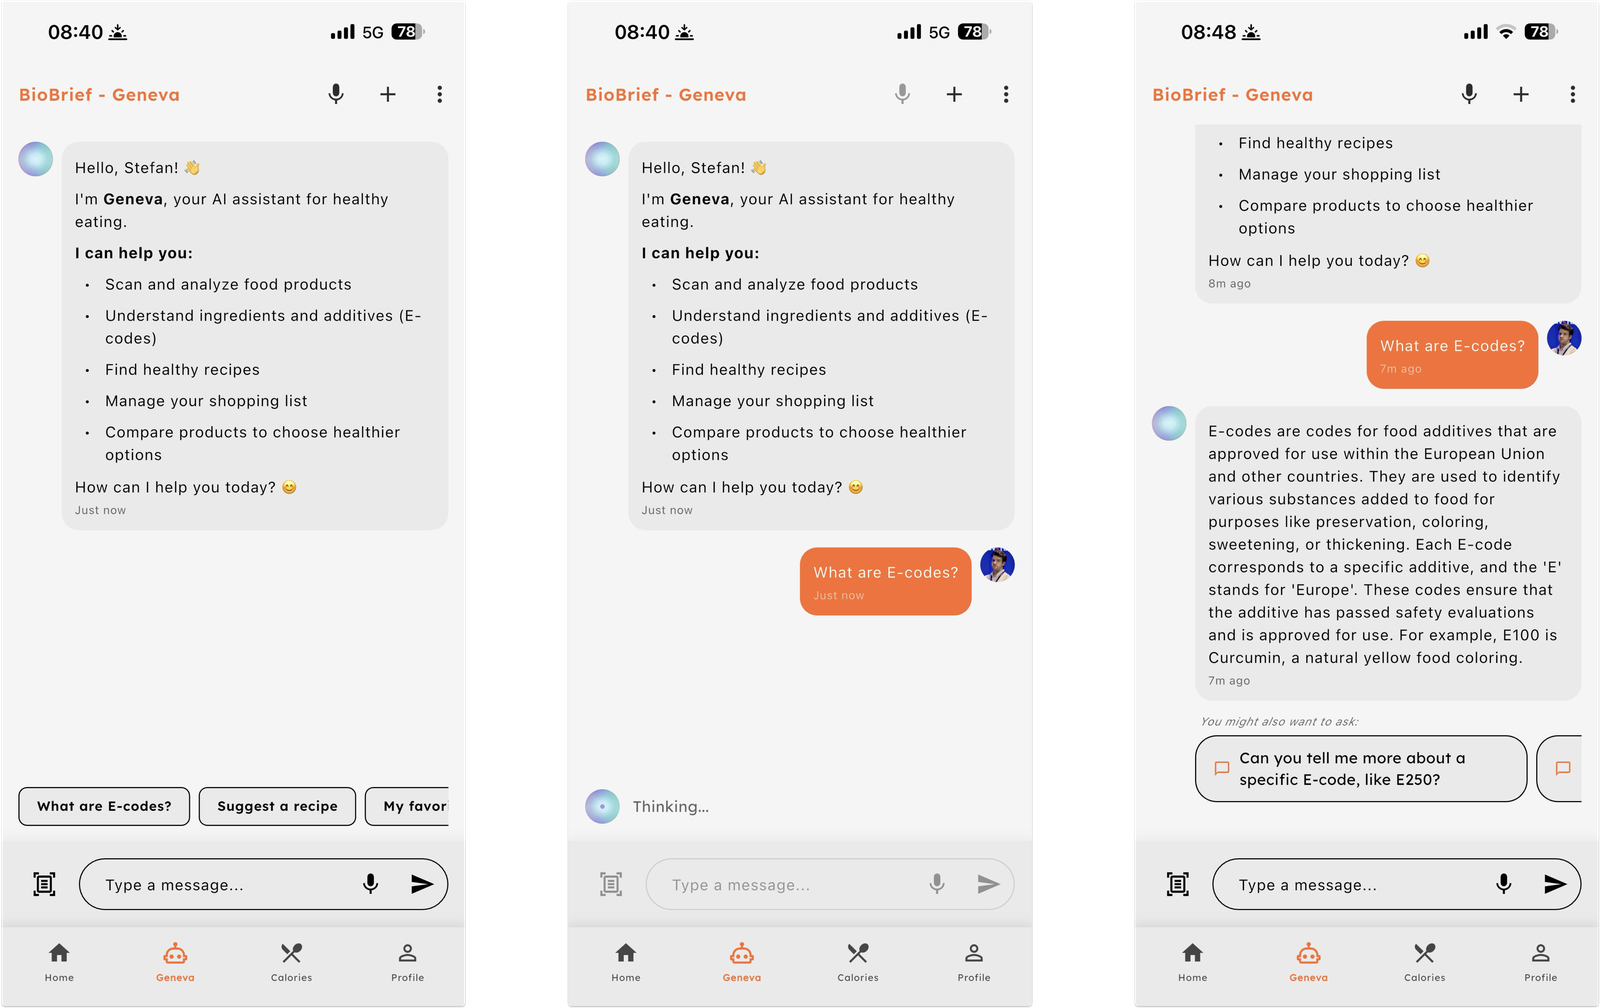
\includegraphics[width=\linewidth,height=46mm,keepaspectratio]{images/onia-s19-1.png}
    \end{column}
    \begin{column}{0.38\textwidth}
      \lead{Say what it can do.}{The first message lists the capabilities. Users do not guess what a text box accepts.}
      \vskip 2mm
      \lead{Offer starters.}{Three suggested questions remove the empty-box problem and teach the vocabulary.}
      \vskip 2mm
      \muted{Follow-up chips keep the conversation inside the part of the app you tested.}
    \end{column}
  \end{columns}
  \note{Point at the thinking state. A local or slow model needs a visible placeholder within one hundred milliseconds or the screen reads as broken, which is a UI problem and not a model problem.}
\end{frame}

\begin{frame}[eyebrow=Conversation]{Hosted model or local model}
  \vskip 1mm
  {\usebeamerfont{small}\begin{tabular}{@{}lp{42mm}p{42mm}@{}}
    \toprule
    \thead{} & \thead{Hosted API} & \thead{Local runtime} \\
    \midrule
    Where it runs & a provider's servers & your laptop, or the phone \\
    Quality       & the strongest models available & smaller models, quantized \\
    Cost          & per token, every call & hardware you already bought \\
    Data          & leaves the device & never leaves the machine \\
    Good for      & production features & demos, tests, sensitive data \\
    \bottomrule
  \end{tabular}}
  \begin{takeaway}{The API surface is the same.}
    Both speak the OpenAI-compatible chat format, so the switch is a base URL and a model id.
  \end{takeaway}
  \note{This is why the demos use a local runtime. The code on the next slides is the code you would ship, with two constants changed.}
\end{frame}

\begin{frame}[eyebrow=Local]{One local endpoint, two models}
  \begin{columns}[T]
    \begin{column}{0.56\textwidth}
      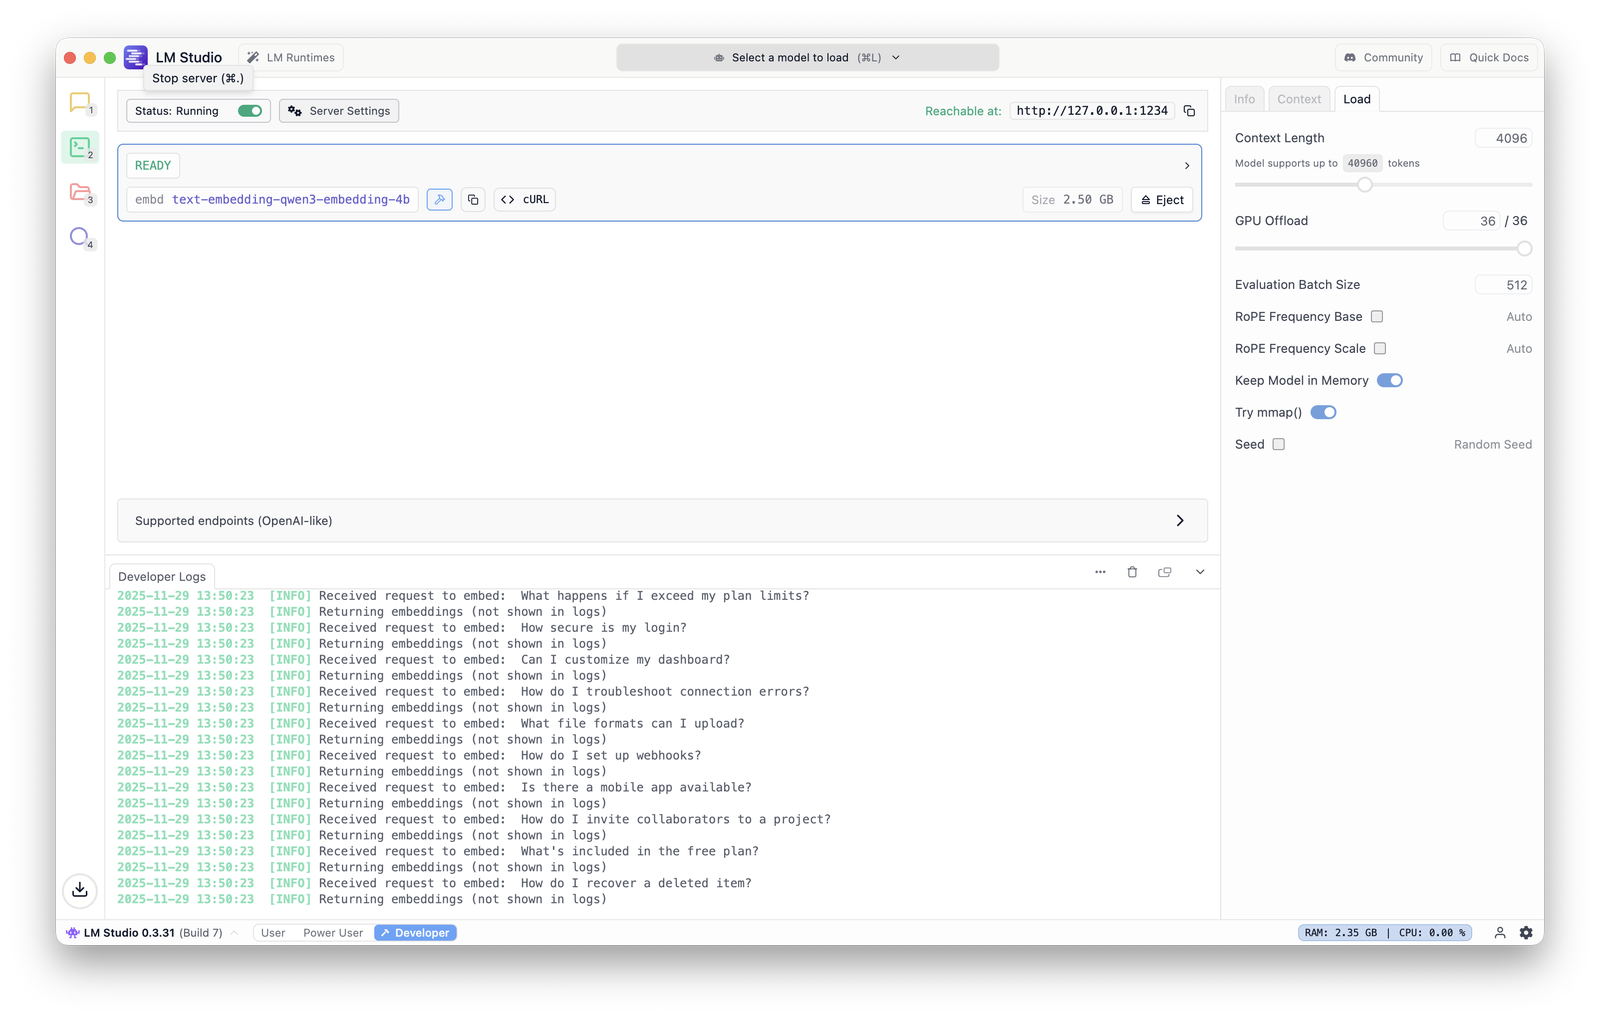
\includegraphics[width=\linewidth,height=44mm,keepaspectratio]{images/rag-s09-1.png}
    \end{column}
    \begin{column}{0.40\textwidth}
      \lead{LM Studio}{A desktop app that downloads open-weight models and serves them over HTTP on \code{127.0.0.1:1234}.}
      \vskip 2mm
      \muted{Load one chat model and one embedding model. The server exposes both on the same OpenAI-compatible paths.}
      \vskip 2mm
      \muted{The developer log shows every request, which makes a failing retrieval step obvious.}
    \end{column}
  \end{columns}
  \note{Show the running server on the real machine if the room is small. Seeing the embedding requests arrive one per document makes the ingestion step concrete later in Part 3.}
\end{frame}

\begin{frame}[fragile,eyebrow=Conversation]{The request shape}
\begin{codeblock}[language=Python]
from openai import OpenAI

client = OpenAI(base_url="http://127.0.0.1:1234/v1", api_key="lm-studio")

response = client.chat.completions.create(
    model="qwen/qwen3.5-9b",
    messages=[{"role": "system", "content": SYSTEM_PROMPT},
              {"role": "user", "content": question}],
    temperature=0.2,
)
\end{codeblock}
  \vskip 1mm
  \muted{A list of messages in, one message out. The model has no memory between calls, so the whole conversation is sent again every turn. That is the bill and the context limit.}
  \note{Say that the system prompt is the only place where you control behavior cheaply. Temperature near zero is the right default for anything that feeds a UI rather than a writing feature.}
\end{frame}

\begin{frame}[fragile,eyebrow=Conversation]{Streaming, and where the key lives}
\begin{codeblock}[language=Python]
stream = client.chat.completions.create(
    model="qwen/qwen3.5-9b", messages=messages, stream=True,
)
for chunk in stream:
    piece = chunk.choices[0].delta.content
    if piece:
        emit(piece)
\end{codeblock}
  \vskip 2mm
  \muted{First token latency is what users call speed. Streaming turns one long wait into an answer that starts at once, and it costs three lines of code.}
  \begin{takeaway}{The key never ships in the app.}
    Anything inside an installed binary is readable. Call your own backend, let it hold the provider key, and hand the app a short-lived user token.
  \end{takeaway}
  \note{Streaming is not decoration. First token latency is what users perceive as speed, and it is often much lower than the time the full completion takes.}
\end{frame}

\divider{Part 3 · Retrieval}{Giving the model your own data}[Embeddings, distance, approximate search, chunking, and a real index]

\begin{frame}[eyebrow=Retrieval]{Why not just send everything}
  \vskip 1mm
  {\usebeamerfont{small}\begin{tabular}{@{}lp{44mm}p{44mm}@{}}
    \toprule
    \thead{} & \thead{Stuff the whole corpus} & \thead{Retrieve, then generate} \\
    \midrule
    Request size & everything you own & the few passages that matter \\
    Result       & rejected, or slow and costly & fits the window easily \\
    Accuracy     & facts get lost in the middle & evidence sits next to the question \\
    Updates      & a new model or a fine-tune & write the document, index it \\
    Auditing     & no idea what was used & you can cite the source file \\
    \bottomrule
  \end{tabular}}
  \begin{takeaway}{Retrieval-augmented generation is a search problem.}
    The model is the last step. Most of the quality comes from what you put in front of it.
  \end{takeaway}
  \note{If someone raises long context windows, agree and then give the real reasons retrieval still wins: cost per call, latency, and the fact that you can point at the paragraph the answer came from.}
\end{frame}

\begin{frame}[eyebrow=Retrieval]{Meaning becomes geometry}
  \begin{columns}[T]
    \begin{column}{0.54\textwidth}
      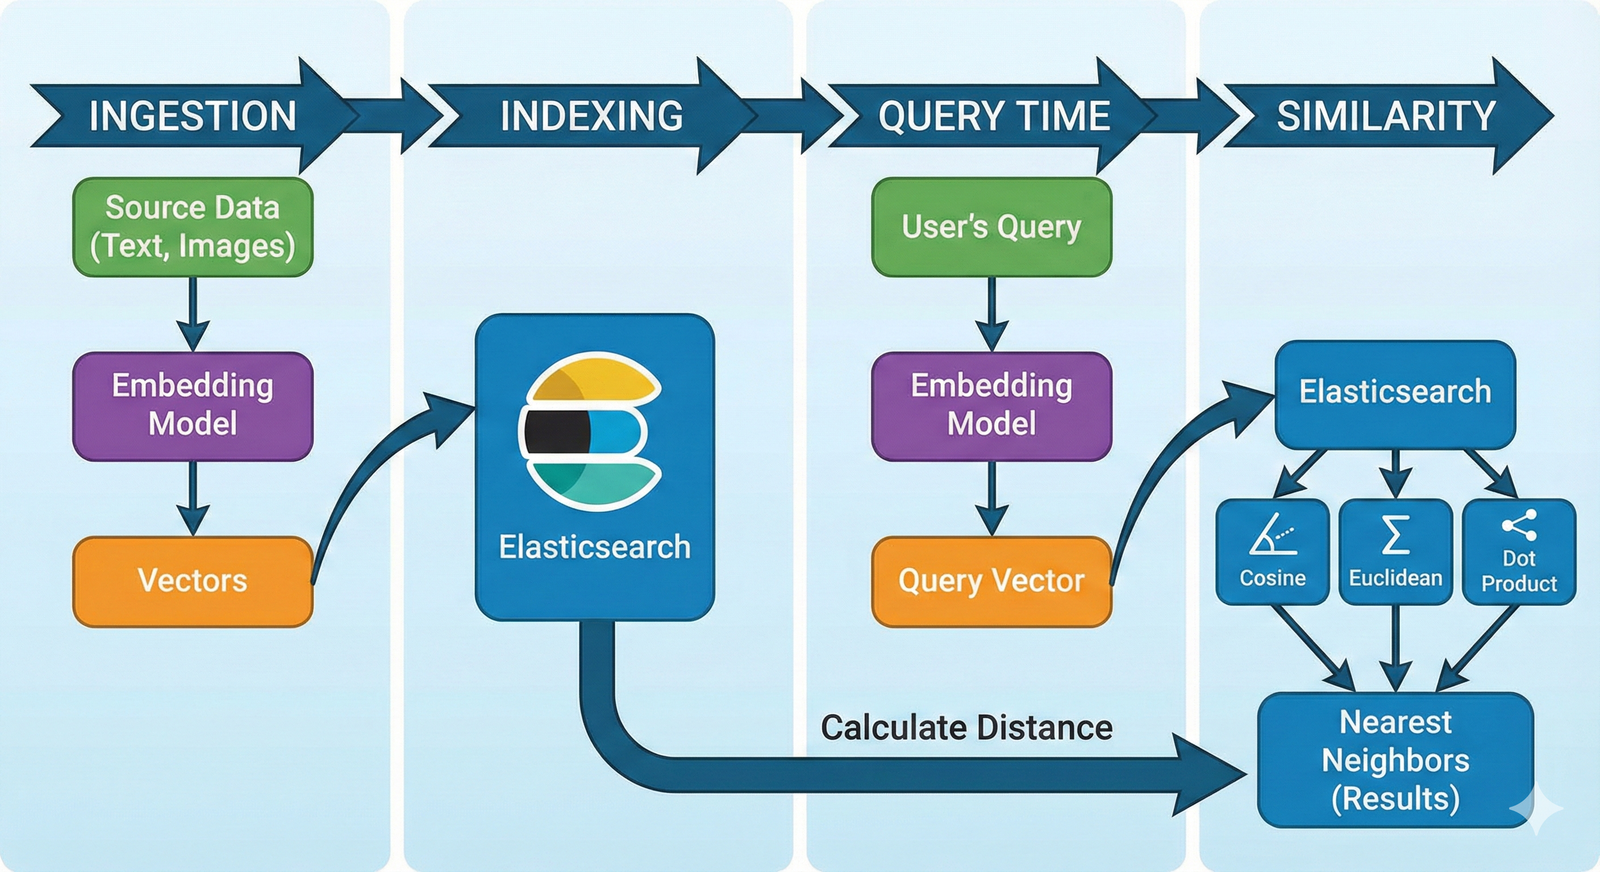
\includegraphics[width=\linewidth,height=42mm,keepaspectratio]{images/rag-s03-1.png}
    \end{column}
    \begin{column}{0.42\textwidth}
      \lead{An embedding is a list of numbers.}{A few hundred to a few thousand floating-point values that place a piece of text in a space.}
      \vskip 2mm
      \muted{Texts about the same thing land close together, even with no shared words. Keyword search cannot do that.}
      \vskip 2mm
      \muted{Documents and questions must go through the same model, or the distances mean nothing.}
    \end{column}
  \end{columns}
  \note{The classic demonstration is king minus man plus woman landing nearest to queen. Use it, then move on quickly: the useful consequence is that a question in Romanian can retrieve an English paragraph.}
\end{frame}

\begin{frame}[eyebrow=Retrieval]{Measuring distance, and finding neighbors}
  \vskip 1mm
  {\usebeamerfont{small}\begin{tabular}{@{}llp{72mm}@{}}
    \toprule
    \thead{Metric} & \thead{Measures} & \multicolumn{1}{l@{}}{\thead{Notes}} \\
    \midrule
    Cosine      & the angle between vectors & ignores length, the safe default for text \\
    Dot product & angle and length together & same ranking as cosine when normalized \\
    Euclidean   & straight-line distance & sensitive to magnitude, used for images \\
    \bottomrule
  \end{tabular}}
  \vskip 2mm
  \muted{Exact search scores every vector and returns the true nearest neighbors, at a cost that grows with the corpus. Approximate search walks a graph of close vectors instead.}
  \begin{takeaway}{Pick the metric the model was trained with, and start exact.}
    A small corpus needs no approximate index.
  \end{takeaway}
  \note{Many models already return normalized vectors, so dot product and cosine give the same order. Name the approximate knobs without dwelling on them: neighbors kept per node, and candidates examined per query.}
\end{frame}

\begin{frame}[eyebrow=Retrieval]{Hybrid search}
  \vskip 2mm
  \begin{grid}[3]
    \cell[\faKey]{Keyword search}{Scores exact term overlap. Unbeatable for product codes, error numbers and names no model has seen.}
    \cell[\faIcon{project-diagram}]{Vector search}{Scores meaning. Finds the paragraph that answers the question in different words.}
    \cell[\faLayerGroup]{Fusion}{Run both, then merge the ranked lists by rank rather than by score, since the scores are not comparable.}
  \end{grid}
  \vskip 3mm
  \begin{takeaway}{Hybrid search fixes the failure each half has on its own.}
    Vector search misses a serial number. Keyword search misses a paraphrase.
  \end{takeaway}
  \note{Give the concrete example from a support corpus: a user pastes an error code and a sentence describing it. The code needs lexical matching and the sentence needs semantic matching, in the same query.}
\end{frame}

\begin{frame}[eyebrow=Retrieval]{Chunking decides what you can retrieve}
  \vskip 2mm
  \begin{grid}[3]
    \cell[\faCut]{Split on structure}{Headings, paragraphs, list items. A chunk that crosses a section boundary answers neither section well.}
    \cell[\faIcon{arrows-alt-h}]{Keep an overlap}{A sentence at the edge belongs to both neighbors. A small overlap stops answers from being cut in half.}
    \cell[\faIcon{tag}]{Carry the metadata}{Store the source file, the section title and the access rules next to the vector, so an answer can be cited.}
  \end{grid}
  \vskip 3mm
  \begin{takeaway}{Chunk size is the main quality knob in a RAG system.}
    Too large and the evidence is diluted. Too small and the passage loses its context.
  \end{takeaway}
  \note{Tell them to measure this rather than guess. Build twenty questions with known answers, then try two or three chunk sizes and count how often the right passage is in the top three.}
\end{frame}

\begin{frame}[eyebrow=Index]{The index, field by field}
  \vskip 2mm
  \begin{center}
    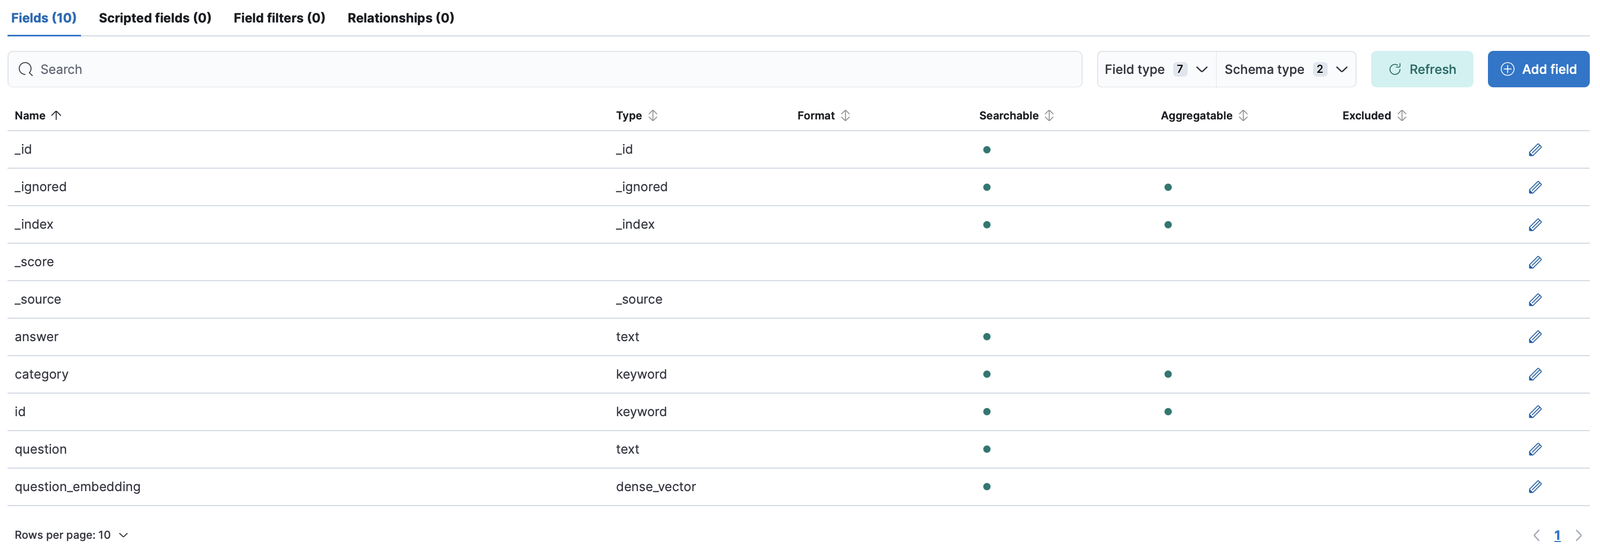
\includegraphics[width=\textwidth,height=26mm,keepaspectratio]{images/rag-s18-1.png}
  \end{center}
  \vskip 2mm
  \muted{A support FAQ index. \code{question} and \code{answer} are analyzed text, \code{category} is a keyword for filtering, and \code{question\_embedding} is a dense vector.}
  \begin{takeaway}{The vector lives next to the text it came from.}
    One query can filter, match keywords and compare vectors at once.
  \end{takeaway}
  \note{Point out that the dimension count is fixed at mapping time. Changing the embedding model means a new field or a new index and a full reindex, so choose it before you load a million documents.}
\end{frame}

\begin{frame}[fragile,eyebrow=Index]{Asking the index a question}
\begin{codeblock}
POST /faqs/_search
{
  "knn": {
    "field": "question_embedding",
    "query_vector": [0.00013, 0.02553, -0.00962, ...],
    "k": 3,
    "num_candidates": 100
  },
  "_source": ["question", "answer", "category"]
}
\end{codeblock}
  \vskip 1mm
  \muted{The query text is embedded by the same model that embedded the documents. Three passages come back with a score, and only those three go into the prompt.}
  \note{Stress the source filter. Returning the raw vector to the app wastes bandwidth and tells an attacker more about your index than you want.}
\end{frame}

\begin{frame}[eyebrow=Demo]{RAG demo}
  \vskip 2mm
  \kv{Notebook}{\code{demos/01\_rag.ipynb}}
  \vskip 1mm
  \begin{enumerate}
    \item Load a small corpus of notes. \muted{Markdown files about this talk and the models.}
    \item Embed and index them. \muted{An in-memory store built with the local embedding model.}
    \item Retrieve and read the distances. \muted{The retrieval step stays visible instead of hiding in a framework.}
    \item Build the prompt and answer. \muted{Answer only from the context, and cite the source file.}
  \end{enumerate}
  \begin{takeaway}{Every model call sits behind a flag that is off by default.}
    The notebook runs end to end with no server.
  \end{takeaway}
  \note{Run the retrieval step first and read the distances out loud before generating anything. When the room sees which passage was chosen, the answer that follows stops looking like magic. Every model call is behind a flag that is off by default.}
\end{frame}

\divider{Part 4 · Tools and MCP}{Letting the model act on your app}[Function calling, MCP servers, and three notebooks]

\begin{frame}[eyebrow=Tools]{The tool calling loop}
  \vskip 2mm
  \begin{enumerate}
    \item You send the tools with the message. \muted{A name, a description and a JSON schema for the arguments.}
    \item The model answers with a call, not with text. \muted{It picks a tool from the descriptions and fills in the arguments.}
    \item Your code runs the tool. \muted{The model never executes anything. It only asks.}
    \item The result goes back as another message. \muted{Tagged with the id of the call it answers.}
    \item The model writes the answer, or calls again. \muted{Cap the rounds, or a confused model will loop.}
  \end{enumerate}
  \begin{takeaway}{The description is the interface.}
    The model chooses a tool by reading its description, so vague descriptions produce wrong calls.
  \end{takeaway}
  \note{Say clearly that steps three and four are your code and your authorization check. Nothing in the protocol stops a model from asking for a tool the current user may not use.}
\end{frame}

\begin{frame}[eyebrow=MCP]{MCP: one protocol between model and app}
  \vskip 2mm
  \begin{center}
    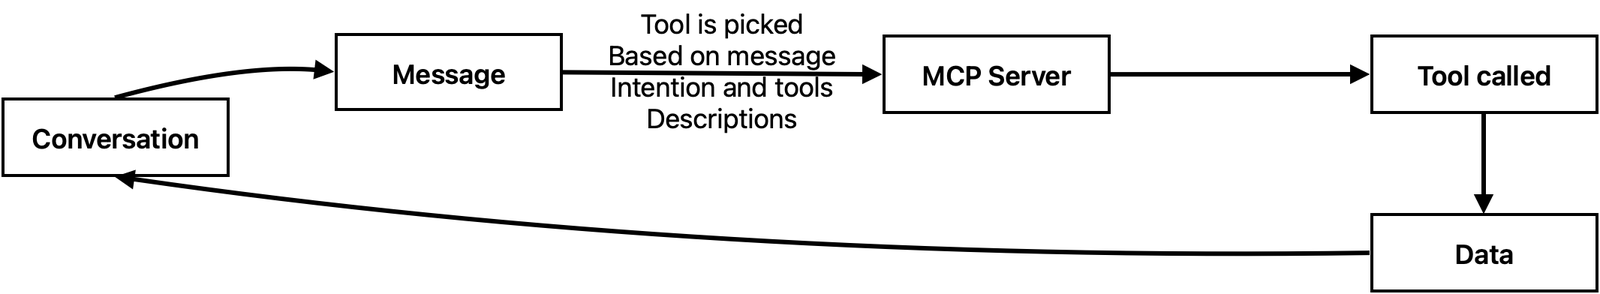
\includegraphics[width=\textwidth,height=22mm,keepaspectratio]{images/onia-s27-1.png}
  \end{center}
  \vskip 3mm
  \muted{The Model Context Protocol standardizes that loop. A server advertises its tools, any compliant client discovers them, and the conversation continues with the result.}
  \begin{takeaway}{Write the integration once.}
    Without MCP you write one tool adapter per client. With it you expose the app once.
  \end{takeaway}
  \note{Make the business point here. An MCP server is a distribution channel: your product becomes reachable from inside the assistant a customer already uses all day.}
\end{frame}

\begin{frame}[fragile,eyebrow=MCP]{Exposing your app as an MCP server}
\begin{codeblock}[language=Python]
from mcp.server import MCPServer

server = MCPServer("recipes")

@server.tool()
def search_recipes(query: str, k: int = 3) -> str:
    """Search the recipe catalog and return matching titles."""
    return "\n".join(catalog.search(query, k))
\end{codeblock}
  \vskip 2mm
  \begin{takeaway}{Your existing service layer is already the tool.}
    The wrapper is a name, a docstring and a typed signature over a function you shipped years ago.
  \end{takeaway}
  \note{Warn about scope. Expose read tools first, keep the argument types narrow, and never let a tool take a raw query string that reaches the database.}
\end{frame}

\begin{frame}[eyebrow=Demo]{MCP demo}
  \vskip 2mm
  {\usebeamerfont{small}\begin{tabular}{@{}llp{56mm}@{}}
    \toprule
    \thead{Notebook} & \thead{Needs} & \multicolumn{1}{l@{}}{\thead{What it shows}} \\
    \midrule
    \code{02\_mcp.ipynb}   & nothing      & three tools, a real client session, discovery and calls over the protocol \\
    \code{03\_agent.ipynb} & local models, internet & retrieval as an MCP tool, live search, a safe page fetcher, one agent loop \\
    \bottomrule
  \end{tabular}}
  \begin{takeaway}{Deterministic when grounding matters, agentic when coverage matters.}
    One path always retrieves and then answers. The other advertises the tool and the model decides.
  \end{takeaway}
  \note{Run the discovery cell first: seeing the tool schemas arrive over a real session, with no model involved, separates the protocol from the model. In notebook 03 the policy in the system prompt sends stable facts to the local index and current facts to the web, and the fetcher refuses private addresses.}
\end{frame}

\divider{Part 5 · Security}{Nothing in this chain is trusted by default}[Input checks, token budgets, human approval, output guardrails]

\begin{frame}[eyebrow=Security]{Before the call: input check and budget}
  \begin{columns}[T]
    \begin{column}{0.54\textwidth}
      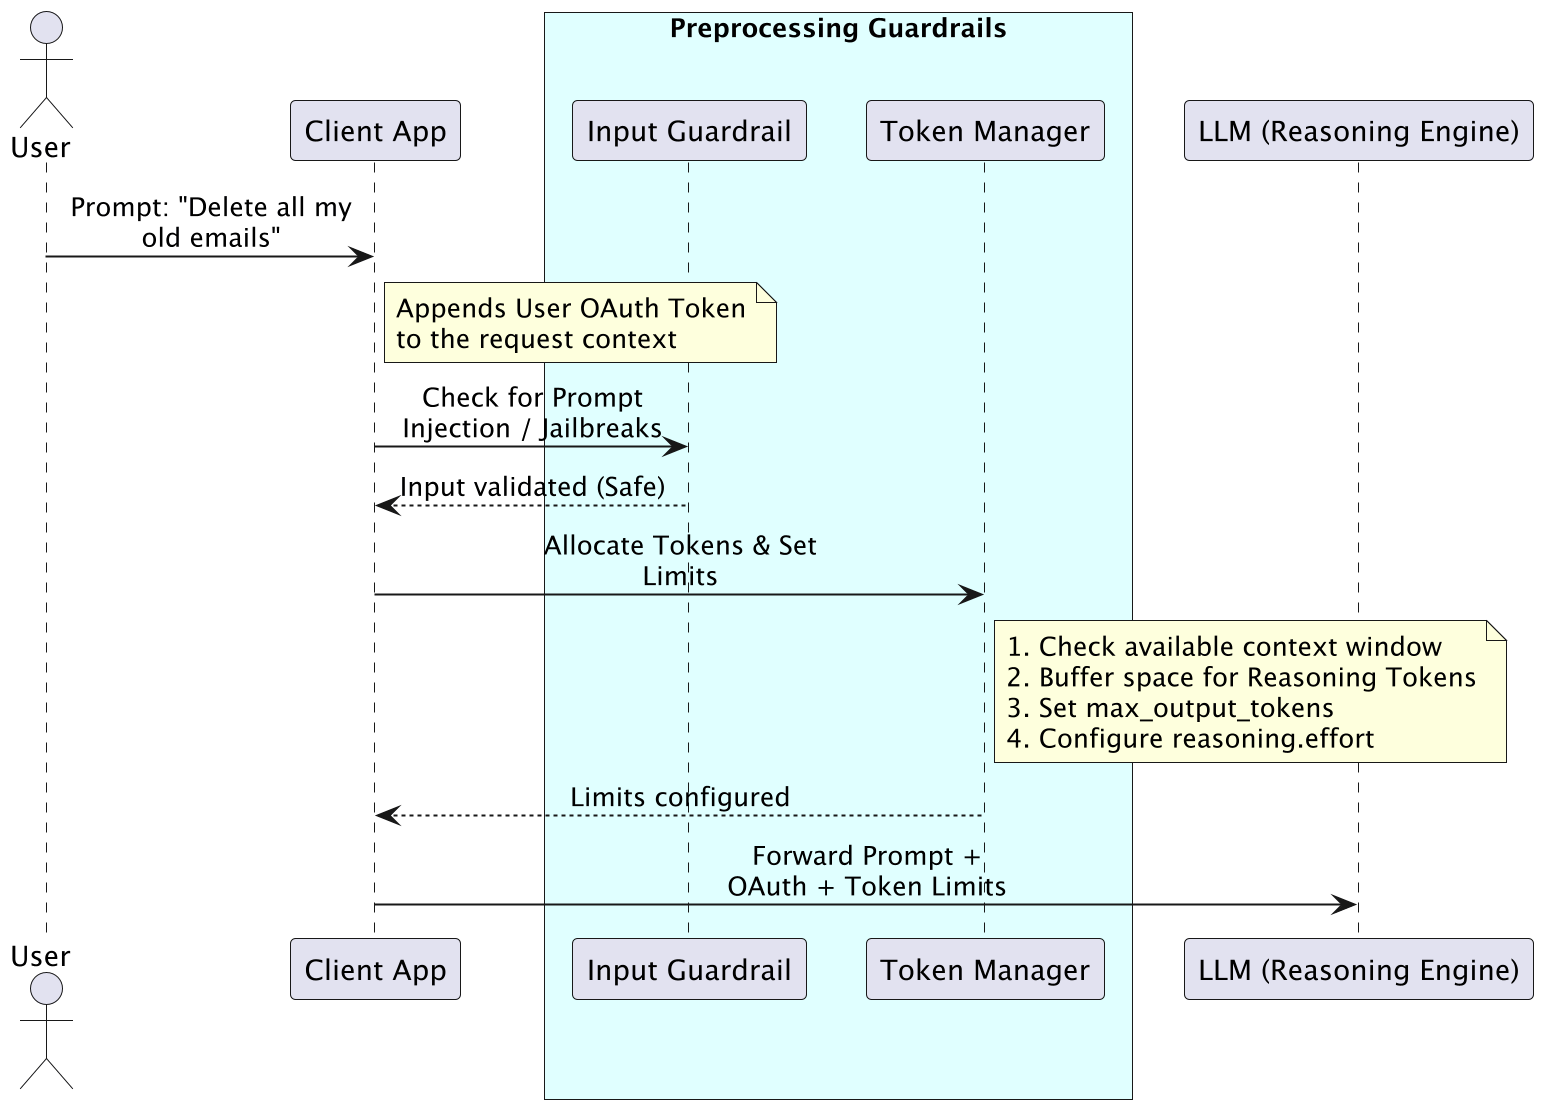
\includegraphics[width=\linewidth,height=44mm,keepaspectratio]{images/onia-s31-1.png}
    \end{column}
    \begin{column}{0.42\textwidth}
      \lead{Attach the user, not a service account.}{The request carries the signed-in user's token, so every tool call runs with that user's rights.}
      \vskip 2mm
      \lead{Check the prompt.}{Screen for injection and jailbreak patterns before the text reaches the model.}
      \vskip 2mm
      \muted{Then set the budget: context left, space reserved for reasoning, a hard cap on output.}
    \end{column}
  \end{columns}
  \note{The token budget is an availability control, not an accounting detail. Without a cap, one crafted prompt can make a reasoning model spend your whole monthly budget on a single answer.}
\end{frame}

\begin{frame}[eyebrow=Security]{Reasoning, validation, human in the loop}
  \vskip 2mm
  \begin{grid}[3]
    \cell[\faIcon{brain}]{Reasoning is not free}{Planning tokens are generated before the answer and spend the same budget. Reserve space for them.}
    \cell[\faCheckDouble]{Validate every call}{The server checks the token scope and the argument schema before anything runs.}
    \cell[\faUserCheck]{Stop for consent}{Deletes, payments and messages pause and ask the user before they happen.}
  \end{grid}
  \vskip 3mm
  \begin{takeaway}{The model proposes. Your server decides.}
    Treat a tool call like a request arriving from a browser you do not control.
  \end{takeaway}
  \note{Give the concrete failure: a prompt hidden inside a document the model just read asks it to delete old records. Schema validation passes, scope validation passes, and only the consent step stops it.}
\end{frame}

\begin{frame}[eyebrow=Security]{Output guardrails}
  \vskip 2mm
  \begin{grid}[3]
    \cell[\faUserSecret]{Check for leaks}{The answer can repeat context the current user was never allowed to see. Scan it before display.}
    \cell[\faIcon{file-signature}]{Check the shape}{If the app expects structured output, parse it and reject what does not fit instead of rendering it.}
    \cell[\faQuoteRight]{Check the citations}{Verify that a cited source was actually in the retrieved set. An invented citation is a confident lie.}
  \end{grid}
  \vskip 3mm
  \begin{takeaway}{Guardrails sit on both ends of the call.}
    One before the model sees the prompt, one before the user sees the answer.
  \end{takeaway}
  \note{Mention logging last. You need the prompt, the retrieved sources and the tool calls to debug a bad answer, and you need to strip personal data from all three before storing them.}
\end{frame}

\begin{frame}[eyebrow=Takeaway]{One thing to take away}
  \vskip 3mm
  \begin{enumerate}
    \item Most of the work is ordinary engineering. \muted{Recognition, normalization, search and validation are code you write and test.}
    \item Retrieval decides the quality, not the model. \muted{Chunk size, metric and metadata move the answer more than a bigger model does.}
    \item Every tool call is untrusted input. \muted{Scope it, validate it, and ask the user before anything irreversible.}
  \end{enumerate}
  \vskip 5mm
  \kv{Demos and slides}{\link{https://rusudinu.ro}{rusudinu.ro} · \link{https://codingshadows.com}{codingshadows.com}}
  \note{Close on the first point. People leave these talks thinking they need a research team, and the honest message is that the hard parts are the ones they already know how to build.}
\end{frame}

\closingframe{Questions?}{rusudinu.ro · codingshadows.com}

\end{document}
